% java -jar /opt/plantuml/plantuml.jar -verbose -tlatex observer.txt; mv observer.latex observer.tex
\begin{figure}[H]	
  \centering
    \resizebox{\linewidth}{!}{\tikzset{font=\Huge}\documentclass{standalone}
\usepackage{tikz}
\usepackage{aeguill}
\begin{document}
% generated by Plantuml 1.2018.12      
\definecolor{plantucolor0000}{RGB}{254,254,206}
\definecolor{plantucolor0001}{RGB}{168,0,54}
\definecolor{plantucolor0002}{RGB}{169,220,223}
\definecolor{plantucolor0003}{RGB}{0,0,0}
\definecolor{plantucolor0004}{RGB}{180,167,229}
\definecolor{plantucolor0005}{RGB}{173,209,178}
\definecolor{plantucolor0006}{RGB}{251,251,119}
\begin{tikzpicture}[yscale=-1
,pstyle0/.style={color=plantucolor0001,fill=plantucolor0000,line width=1.5pt}
,pstyle2/.style={color=plantucolor0001,line width=1.5pt}
,pstyle4/.style={color=plantucolor0001,fill=plantucolor0005,line width=1.0pt}
,pstyle5/.style={color=plantucolor0001,fill=plantucolor0006,line width=1.0pt}
,pstyle6/.style={color=plantucolor0001,line width=1.0pt}
,pstyle7/.style={color=plantucolor0001,fill=plantucolor0001,line width=1.0pt}
]
\draw[pstyle0] (62pt,109pt) rectangle (190.3385pt,221.0234pt);
\draw[color=plantucolor0001,fill=plantucolor0002,line width=1.0pt] (96.3127pt,125pt) ellipse (11pt and 11pt);
\node at (96.3127pt,125pt)[]{\textbf{\Large A}};
\node at (114.6045pt,118.0156pt)[below right,color=black]{\textit{Subject}};
\draw[pstyle2] (63pt,141pt) -- (189.3385pt,141pt);
\node at (68pt,145pt)[below right,color=black]{+observers};
\draw[pstyle2] (63pt,161.8047pt) -- (189.3385pt,161.8047pt);
\node at (68pt,165.8047pt)[below right,color=black]{+attach(o : Obs)};
\node at (68pt,178.6094pt)[below right,color=black]{+detach(o : Obs)};
\node at (68pt,191.4141pt)[below right,color=black]{+notifyObs()};
\node at (68pt,204.2188pt)[below right,color=black]{\textit{getSubjectStatus()}};
\draw[pstyle0] (298.5pt,134.5pt) rectangle (395.7421pt,195.3047pt);
\draw[color=plantucolor0001,fill=plantucolor0004,line width=1.0pt] (313.5pt,150.5pt) ellipse (11pt and 11pt);
\node at (313.5pt,150.5pt)[]{\textbf{\Large I}};
\node at (327.5pt,143.5156pt)[below right,color=black]{\textit{Observer}};
\draw[pstyle2] (299.5pt,166.5pt) -- (394.7421pt,166.5pt);
\draw[pstyle2] (299.5pt,174.5pt) -- (394.7421pt,174.5pt);
\node at (304.5pt,178.5pt)[below right,color=black]{\textit{update()}};
\draw[pstyle0] (73pt,282pt) rectangle (222.8118pt,342.8047pt);
\draw[pstyle4] (88pt,298pt) ellipse (11pt and 11pt);
\node at (88pt,298pt)[]{\textbf{\Large C}};
\node at (102pt,291.0156pt)[below right,color=black]{ConcreteSubject};
\draw[pstyle2] (74pt,314pt) -- (221.8118pt,314pt);
\draw[pstyle2] (74pt,322pt) -- (221.8118pt,322pt);
\node at (79pt,326pt)[below right,color=black]{getSubjecdtStatus()};
\draw[pstyle0] (262.5pt,282pt) rectangle (423.9pt,342.8047pt);
\draw[pstyle4] (277.5pt,298pt) ellipse (11pt and 11pt);
\node at (277.5pt,298pt)[]{\textbf{\Large C}};
\node at (291.5pt,291.0156pt)[below right,color=black]{ConcreteObserver};
\draw[pstyle2] (263.5pt,314pt) -- (422.9pt,314pt);
\draw[pstyle2] (263.5pt,322pt) -- (422.9pt,322pt);
\node at (268.5pt,326pt)[below right,color=black]{update()};
\draw[pstyle5] (284.5pt,8pt) -- (284.5pt,48.2656pt) -- (343pt,48.2656pt) -- (347pt,134.2998pt) -- (351pt,48.2656pt) -- (409.4636pt,48.2656pt) -- (409.4636pt,18pt) -- (399.4636pt,8pt) -- (284.5pt,8pt);
\draw[pstyle5] (399.4636pt,8pt) -- (399.4636pt,18pt) -- (409.4636pt,18pt) -- (399.4636pt,8pt);
\node at (290.5pt,13pt)[below right,color=black]{may be an};
\node at (290.5pt,28.1328pt)[below right,color=black]{abstract class};
\draw[pstyle5] (6pt,15.5pt) -- (6pt,40.6328pt) -- (122pt,40.6328pt) -- (126pt,108.8568pt) -- (130pt,40.6328pt) -- (245.8pt,40.6328pt) -- (245.8pt,25.5pt) -- (235.8pt,15.5pt) -- (6pt,15.5pt);
\draw[pstyle5] (235.8pt,15.5pt) -- (235.8pt,25.5pt) -- (245.8pt,25.5pt) -- (235.8pt,15.5pt);
\node at (12pt,20.5pt)[below right,color=black]{may be interface or concrete};
\draw[pstyle6] (203.2192pt,165pt) ..controls (203.2192pt,165pt) and (285.4477pt,165pt) .. (285.4477pt,165pt);
\draw[pstyle7] (298.4477pt,165pt) -- (289.4477pt,161pt) -- (293.4477pt,165pt) -- (289.4477pt,169pt) -- (298.4477pt,165pt) -- cycle;
\draw[pstyle6] (293.4477pt,165pt) -- (285.4478pt,165pt);
\draw[pstyle7] (190.2192pt,165pt) -- (196.2192pt,169pt) -- (202.2192pt,165pt) -- (196.2192pt,161pt) -- (190.2192pt,165pt) -- cycle;
\draw[pstyle6] (131.5pt,241.1842pt) ..controls (131.5pt,241.1842pt) and (131.5pt,281.6437pt) .. (131.5pt,281.6437pt);
\draw[pstyle6] (124.5001pt,241.1842pt) -- (131.5pt,221.1842pt) -- (138.5001pt,241.1842pt) -- (124.5001pt,241.1842pt) -- cycle;
\draw[color=plantucolor0001,line width=1.0pt,dash pattern=on 7.0pt off 7.0pt] (347pt,215.5621pt) ..controls (347pt,215.5621pt) and (347pt,281.9771pt) .. (347pt,281.9771pt);
\draw[pstyle6] (340.0001pt,215.5621pt) -- (347pt,195.5621pt) -- (354.0001pt,215.5621pt) -- (340.0001pt,215.5621pt) -- cycle;
\draw[pstyle6] (223.1132pt,313pt) ..controls (223.1132pt,313pt) and (257.4237pt,313pt) .. (257.4237pt,313pt);
\draw[pstyle7] (262.4237pt,313pt) -- (253.4237pt,309pt) -- (257.4237pt,313pt) -- (253.4237pt,317pt) -- (262.4237pt,313pt) -- cycle;
\end{tikzpicture}
\end{document}
}
\end{figure}
\begin{intentbox}[Intent]\nospacing
  \begin{itemize}
      \item Consistency assurance between cooperating objects without connecting them too much.
      \item  One-to-many relation between objects which allows to inform the
        dependent objects about state changes
  \end{itemize}
\end{intentbox}
\begin{codeboxNl}[Observer]{java}
  interface Observer{
    void update ();
  }
\end{codeboxNl}
\begin{codeboxNl}[Subject]{java}
class Subject {
  private List <Observer > observers = new ArrayList <Observer >();

  public void addObserver(Observer o) {
    // method of List
    observers.add(o);
  }

  public void removeObserver(Observer o) {
    // method of List
    observers.remove(o);
  }

  protected void notifyObservers () {
    // inform all Observers that we have changed
    for(Observer obs : observers) {
      // Let (concrete) observers handle it
      obs.|\ul{update}| ();
    }
  }
}
\end{codeboxNl}
\begin{codeboxNl}[Concrete Subject]{java}
class ConcSubject extends Subject {
  private int state;
  public int getState (){
    return state;
  }

  public void setState(int val){
    state = val;
    notifyObservers();
  }
}
\end{codeboxNl}
\begin{codeboxNl}[Concrete Observer]{java}
class ConcObserver implements Observer {
  private |\ul[ulc4]{ConcSubject s}|;
  ConcObserver (ConcSubject s){
    this.s = s;
    s.addObserver(this);
  }

  public void |\ul{update}| (){
    // take appropriate steps
  }
}
\end{codeboxNl}
\begin{partbox}[Participants]\nospacing
  \begin{itemizenosep}
      \item \imp{Observer}: typically an interface that declares methods to
      handle notifications.
      \item \imp{Subject}: maybe concrete or interface knows its observers over
      the observer interface (guarantee that the method \ul{\javainline{update}}
      exists).
        \item \imp{Concrete Observer}:
      \begin{itemize}
          \item Handles state changes of its observable
          \item Implements the observer interface to keep its state consistent with
                the subject
          \item May maintain a \ul[ulc4]{reference} to a concrete subject (pull-model)
        \todo[inline]{Check if ref is really because of pull model}
      \end{itemize}
      \item \imp{Concrete Subject}: Implements/extends Subject and hence can:
      \begin{itemize}
          \item attach observers
          \item detach observers
          \item call the method notify if its state changes\\
          (e.g.\ in a set method)
      \end{itemize}
  \end{itemizenosep}
\end{partbox}
\begin{consequencebox}[Consequence]
  \begin{itemizenosep}
    \item Subject does not care about the number of observers $\Rightarrow$
    notifications are broadcast.
    \item A simple state change/operation may lead to a (unwanted) cascade of
  updates.\\
  $\rightarrow$ beware of cyclic dependencies see
  \todo[inline]{add cref}
  \end{itemizenosep}
\end{consequencebox}
\begin{notebox}[Note]\nospacing
  \begin{itemizenosep}
      \item Thus it is up to the observer to handle or \imp{ignore}
    notifications.
      \item When should \javainline{notifyObservers} be called?
    \begin{itemizenosep}
        \item \imp{Automatically}: at every state change\\
      $\Rightarrow$ many updates
        \item \imp{Explicitly}: after a set of changes\\
      $\Rightarrow$ responsibility e.g.\
      \begin{itemize}
          \item Asynchronous at idle times 
          \item Use a boolean flag \javainline{changed}, that can be set in
          order to test if object has changed see \cref{subsubsec:Java.util.Observable}
        \todo[inline]{clarify why or what for?}
      \end{itemize}
    \end{itemizenosep}
  \end{itemizenosep}
\end{notebox}
\subsubsection{One or Many Observables}
\begin{figure}[H]	
  \centering
  \resizebox{\linewidth}{!}{\tikzset{font=\Huge}\documentclass{standalone}
\usepackage{tikz}
\usepackage{aeguill}
\begin{document}
% generated by Plantuml 1.2018.12      
\definecolor{plantucolor0000}{RGB}{254,254,206}
\definecolor{plantucolor0001}{RGB}{168,0,54}
\definecolor{plantucolor0002}{RGB}{169,220,223}
\definecolor{plantucolor0003}{RGB}{0,0,0}
\definecolor{plantucolor0004}{RGB}{3,128,72}
\definecolor{plantucolor0005}{RGB}{132,190,132}
\definecolor{plantucolor0006}{RGB}{180,167,229}
\definecolor{plantucolor0007}{RGB}{255,0,0}
\begin{tikzpicture}[yscale=-1
,pstyle0/.style={color=plantucolor0001,fill=plantucolor0000,line width=1.5pt}
,pstyle2/.style={color=plantucolor0001,line width=1.5pt}
,pstyle4/.style={color=plantucolor0004,fill=plantucolor0005,line width=1.0pt}
]
\draw[pstyle0] (6pt,8pt) rectangle (148.3385pt,120.0234pt);
\draw[color=plantucolor0001,fill=plantucolor0002,line width=1.0pt] (34.138pt,24pt) ellipse (11pt and 11pt);
\node at (34.138pt,24pt)[]{\textbf{\Large A}};
\node at (51.0576pt,17.0156pt)[below right,color=black]{\textit{Observable}};
\draw[pstyle2] (7pt,40pt) -- (147.3385pt,40pt);
\draw[color=plantucolor0004,line width=1.0pt] (17pt,51.9023pt) ellipse (3pt and 3pt);
\node at (26pt,44pt)[below right,color=black]{observers};
\draw[pstyle2] (7pt,60.8047pt) -- (147.3385pt,60.8047pt);
\draw[pstyle4] (17pt,72.707pt) ellipse (3pt and 3pt);
\node at (26pt,64.8047pt)[below right,color=black]{attach(o : Obs)};
\draw[pstyle4] (17pt,85.5117pt) ellipse (3pt and 3pt);
\node at (26pt,77.6094pt)[below right,color=black]{detach(o : Obs)};
\draw[pstyle4] (17pt,98.3164pt) ellipse (3pt and 3pt);
\node at (26pt,90.4141pt)[below right,color=black]{notifyObs()};
\node at (26pt,103.2188pt)[below right,color=black]{\textit{getSubjectStatus()}};
\draw[pstyle0] (268.5pt,33.5pt) rectangle (365.7421pt,94.3047pt);
\draw[color=plantucolor0001,fill=plantucolor0006,line width=1.0pt] (283.5pt,49.5pt) ellipse (11pt and 11pt);
\node at (283.5pt,49.5pt)[]{\textbf{\Large I}};
\node at (297.5pt,42.5156pt)[below right,color=black]{\textit{Observer}};
\draw[pstyle2] (269.5pt,65.5pt) -- (364.7421pt,65.5pt);
\draw[pstyle2] (269.5pt,73.5pt) -- (364.7421pt,73.5pt);
\node at (274.5pt,77.5pt)[below right,color=black]{\textit{update()}};
\draw[color=plantucolor0001,line width=1.0pt] (148.0338pt,64pt) ..controls (148.0338pt,64pt) and (263.2019pt,64pt) .. (263.2019pt,64pt);
\draw[color=plantucolor0001,fill=plantucolor0001,line width=1.0pt] (268.2019pt,64pt) -- (259.2019pt,60pt) -- (263.2019pt,64pt) -- (259.2019pt,68pt) -- (268.2019pt,64pt) -- cycle;
\node at (163.6179pt,65pt)[below right,color=black]{observers};
\draw[color=black,fill=black,line width=1.0pt] (238.5064pt,71.0664pt) -- (244.5064pt,74.0664pt) -- (238.5064pt,77.0664pt) -- (238.5064pt,71.0664pt) -- cycle;
\node at (156.2823pt,48.1933pt)[below right,color=plantucolor0007]{\textbf{?}};
\node at (252.5886pt,47.785pt)[below right,color=black]{*};
\end{tikzpicture}
\end{document}
}
\end{figure}
\begin{sectionbox}[0\ldots 1 : *]\nospacing
  \begin{itemizenosep}
      \item Subject/Observable is usually passed to constructor of the Concrete
    Observer ($\Rightarrow$ \ul[ulc4]{reference}).
      \item 
  \end{itemizenosep}
\end{sectionbox}
\begin{sectionbox}[* : *]\nospacing
  \begin{itemizenosep}
      \item If we want that observers can observe multiple subjects and if these
    observers may be able to ignore certain events from those subjects,
    then the observer need to know the source of an update event.\\
    Moreover if arguments are passed to the Observables, then the observer needs
    to know:
    \begin{itemize}
        \item The arguments
        \item The source of the event
    \end{itemize}
  \end{itemizenosep}
\end{sectionbox}
\begin{figure}[H]	
  \centering
  \resizebox{\linewidth}{!}{\tikzset{font=\Huge}\documentclass{standalone}
\usepackage{tikz}
\usepackage{aeguill}
\begin{document}
% generated by Plantuml 1.2018.12      
\definecolor{plantucolor0000}{RGB}{254,254,206}
\definecolor{plantucolor0001}{RGB}{168,0,54}
\definecolor{plantucolor0002}{RGB}{169,220,223}
\definecolor{plantucolor0003}{RGB}{0,0,0}
\definecolor{plantucolor0004}{RGB}{3,128,72}
\definecolor{plantucolor0005}{RGB}{132,190,132}
\definecolor{plantucolor0006}{RGB}{255,0,0}
\definecolor{plantucolor0007}{RGB}{180,167,229}
\begin{tikzpicture}[yscale=-1
,pstyle0/.style={color=plantucolor0001,fill=plantucolor0000,line width=1.5pt}
,pstyle2/.style={color=plantucolor0001,line width=1.5pt}
,pstyle4/.style={color=plantucolor0004,fill=plantucolor0005,line width=1.0pt}
]
\draw[pstyle0] (6pt,8pt) rectangle (170.5237pt,120.0234pt);
\draw[color=plantucolor0001,fill=plantucolor0002,line width=1.0pt] (44.1214pt,24pt) ellipse (11pt and 11pt);
\node at (44.1214pt,24pt)[]{\textbf{\Large A}};
\node at (63.2595pt,17.0156pt)[below right,color=black]{\textit{Observable}};
\draw[pstyle2] (7pt,40pt) -- (169.5237pt,40pt);
\draw[color=plantucolor0004,line width=1.0pt] (17pt,51.9023pt) ellipse (3pt and 3pt);
\node at (26pt,44pt)[below right,color=black]{observers};
\draw[pstyle2] (7pt,60.8047pt) -- (169.5237pt,60.8047pt);
\draw[pstyle4] (17pt,72.707pt) ellipse (3pt and 3pt);
\node at (26pt,64.8047pt)[below right,color=black]{attach(o : Obs)};
\draw[pstyle4] (17pt,85.5117pt) ellipse (3pt and 3pt);
\node at (26pt,77.6094pt)[below right,color=black]{detach(o : Obs)};
\draw[pstyle4] (17pt,98.3164pt) ellipse (3pt and 3pt);
\node at (26pt,90.4141pt)[below right,color=black]{notifyObs(};
\node at (90.2207pt,90.4141pt)[below right,color=plantucolor0006]{Object args};
\node at (159.7237pt,90.4141pt)[below right,color=black]{)};
\node at (26pt,103.2188pt)[below right,color=black]{\textit{getSubjectStatus()}};
\draw[pstyle0] (206.5pt,27pt) rectangle (398.3264pt,100.6094pt);
\draw[color=plantucolor0001,fill=plantucolor0007,line width=1.0pt] (265.5422pt,43pt) ellipse (11pt and 11pt);
\node at (265.5422pt,43pt)[]{\textbf{\Large I}};
\node at (286.0422pt,36.0156pt)[below right,color=black]{\textit{Observer}};
\draw[pstyle2] (207.5pt,59pt) -- (397.3264pt,59pt);
\draw[pstyle2] (207.5pt,67pt) -- (397.3264pt,67pt);
\node at (212.5pt,71pt)[below right,color=black]{\textit{update(}};
\node at (212.5pt,83.8047pt)[below right,color=plantucolor0006]{\textit{Observable src, Object args}};
\node at (387.5264pt,83.8047pt)[below right,color=black]{\textit{)}};
\draw[color=plantucolor0001,line width=1.0pt] (171.238pt,65pt) ..controls (171.238pt,65pt) and (201.4327pt,65pt) .. (201.4327pt,65pt);
\draw[color=plantucolor0001,fill=plantucolor0001,line width=1.0pt] (206.4327pt,65pt) -- (197.4327pt,61pt) -- (201.4327pt,65pt) -- (197.4327pt,69pt) -- (206.4327pt,65pt) -- cycle;
\node at (178.4336pt,49.4662pt)[below right,color=black]{*};
\node at (190.6096pt,49.4444pt)[below right,color=black]{*};
\end{tikzpicture}
\end{document}
}
\end{figure}
\begin{codeboxNl}[Many vs Many]{java}
protected void notifyObservers(Object args){
    for(Observer obs : observers){
        obs.update(this, args);
    }
}
\end{codeboxNl}
\subsubsection{Push vs Pull Model}
\begin{sectionbox}[\tc{section}{Push-Model}]\nospacing
  \begin{itemizenosep}
      \item The subject (i.e.\ the Observable) sends the observer on notification all the data it will need.
      The observer doesn't need to query the subject for information.
      \item Observable must know which information is needed by the observers
      in order for them to act appropriately (or Observable sends all data)
  \end{itemizenosep}
\end{sectionbox}
\begin{sectionbox}[\tc{section}{Pull-Model}]\nospacing
  \begin{itemizenosep}
      \item 
      In the pull model, the subject merely notifies the observer that something
      happened, and the observer queries the subject based on that, to get the information it needs.
      \item Observable send only information about what has changed
      \item Observer has to access the Observable state (via \ul[ulc4]{reference})
  \end{itemizenosep}
\end{sectionbox}
\todo[inline]{maybe add pros and cons}
\subsection*{Pitfalls}
\label{subsubsec:Pitfalls}
\subsubsection{Java.util.Observable}
\label{subsubsec:Java.util.Observable}
\begin{sectionbox}\nospacing
  Provides an implementation of an Observable that can be used.\\
  \imp{But} it is never used!\\
  \imp{Problem}: multiple inheritance is in java not possible, thus
  \javainline{Java.util.Observable} can only be implemented if extension is not
  defined in its own inheritance hierarchy.\\
  \imp{Solution}: \tc{section}{composite} twin class (\cref{subsection:Composite}).\\
    $\Rightarrow$ code duplication $\Rightarrow$ \javainline{Java.util.Observable}
  is not used.
\end{sectionbox}
\begin{codeboxNl}[\texttt{Java.util.Observable}]{java}
public interface Observer {
  void update(Observable o, Object arg);
}

public class Observable {
  private boolean changed = false;

  // Marks this Observable as having been changed
  protected void setChanged() { changed = true; }

  // Indicates that this object has no longer changed,
  // or that it has already notified all of its observers
  // of its most recent change.
  protected void clearChanged() { changed = false; }

  // Tests if this object has changed.
  public boolean hasChanged() { return changed; }

  // If this object has changed, as indicated by the
  // hasChanged method, then notify all of its observers
  // and then call the clearChanged method to indicate
  // that this object has no longer changed.
  public void notifyObservers(Object arg) {
    if (!changed) return;
    // See section on ConcurrentModificationException
    Object[] copy = obs.toArray();
    clearChanged(); // before notification!
    for (int i = copy.length-1; i>=0; i--)
      ((Observer)copy[i]).update(this, arg);
  }
}
\end{codeboxNl}
\todo[inline]{Add observable twin class solution after we studied again composite}
\subsubsection{ConcurrentModificationException}
\label{subsubsec:ConcurrentModificationException}
\begin{defnbox}\nospacing
  \begin{defn}[\javainline{ConcurrentModificationException}]
    We cannot change a list e.g.\ add/remove while iterating over it.\\
    \imp{Example}: Once Observer and notify.
  \end{defn}
\end{defnbox}
\begin{defnbox}\nospacing
  \begin{defn}[OnceObserver]\label{defn:OnceObserver}
    Is an observer that only observers for a single notification.\\
    $\Rightarrow$ removes itself afterwards.
  \end{defn}
\end{defnbox}
\begin{codeboxNl}[OnceObserver]{java}
public class OnceObserver implements Observer {
  public void update(Observable |$\overbrace{\text{source}}^{\mathclap{\text{Conc. Observerable}}}$|, Object arg) {
        // take appropriate steps once
        source.|\ul[ulc5]{removeObserver}|(this);
  }
}
\end{codeboxNl}
\begin{codeboxcomment}[Problem]{0.74}{java}{\imp{Problem}: we cannot remove an
    observer from \javainline{obs} while iterating over it}
protected void notifyObservers(Object arg){
  for(Observer obs : observers){
    obs.update(this, arg);
  }
}
\end{codeboxcomment}
\begin{sectionbox}[Solutions]\nospacing
  \begin{circlelistnosep}
      \item Perform the notifications on a copy of the observer list.
      \item Delay add/remove Observer calls.
      \item Copy the observer list upon modification.
  \end{circlelistnosep}
\end{sectionbox}
\begin{defnbox}\nospacing
  \begin{defn}[Java list to array]
    Returns an array containing all of the elements in this list in proper sequence (from first to last element).
    \begin{mintlinebox}{java}
      java.util.ArrayList.toArray(a T[])
    \end{mintlinebox}
    \javainline{a}: is the array into which the elements of the list are to be
    stored, if it is big enough; otherwise, a new array of the same runtime type is allocated for this purpose.
  \end{defn}
\end{defnbox}
\todo[inline]{understand better how this works}
\begin{codeboxNl}[Copy Solution]{java}
protected void notifyObservers(){
  Observer[] copy;
  copy = observers.toArray(new Observer[observers.size()]);
  for (Observer obs : copy){
    obs.update(this);
  }
}
\end{codeboxNl}
\begin{codeboxNl}[Alternative]{java}
protected void notifyObservers(){
  for(Observer o : new ArrayList<>(observables)){
    o.update(this);
  }
}
\end{codeboxNl}
\todo[inline]{maybe add Mutation or gamble, must likly not important}
\begin{defnbox}\nospacing
  \begin{defn}[Copy on write list]
    Thread-safe variant of ArrayList in which
    all mutative operations are implemented by making a fresh copy of the
    underlying array.
  \end{defn}
\end{defnbox}
\begin{codeboxNl}[Best Solution]{java}
  private List<Observer> observers = new CopyOnWriteArrayList<>();
  public void addObserver(Observer o) { observers.add(o); }
  public void removeObserver(Observer o) { observers.remove(o); }

  protected void notifyObservers(Object arg) {
    for(Observer obs : observers) {
      obs.update(this, arg);
    }
  }
\end{codeboxNl}
\subsubsection{Cyclic dependencies}
\label{subsubsec:CyclicDependencies}
\begin{sectionbox}[Problem]\nospacing
  If we have a cyclic dependency we will end up in an endless loop of notifying
  and updating, unless we take appropriate measures.
\begin{figure}[H]
  \centering
  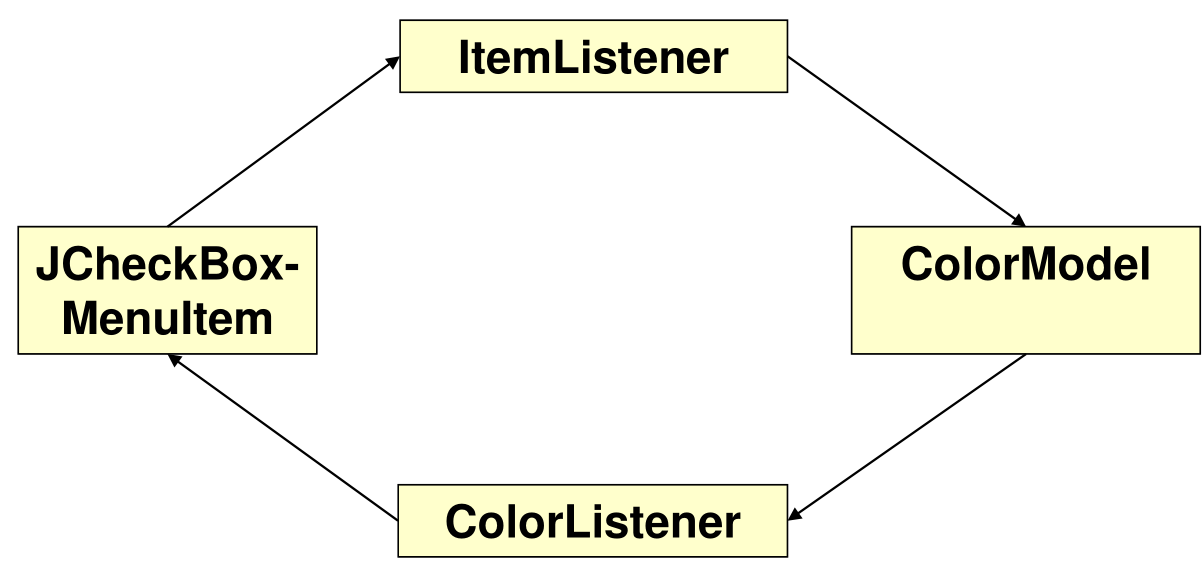
\includegraphics[width=0.7\columnwidth]{figures/cyclic_dependency.png}
  \label{fig:cyclic_dependency}
\end{figure}
\imp{General Rule}: Propagate changes only if the model really changed!
\end{sectionbox}
\begin{sectionbox}[Solution 1: Color Listener]\nospacing
    Break recursion inside the listener: e.g.\ we
    check inside the color listener if the color really changed, or is still the
    same $\Rightarrow$ recursion or nothing happens anyway.
      \begin{mintlinebox}{java}
        // update method of listener
       public void colorValueChanged(Color c){
          if (isSelected() OR_OPRATOR !c.equals(this.color))
          // If the color really changed and isSelected is true
          // select the checkbox menu item
            setSelected(c.equals(this.color));
        }
      \end{mintlinebox}
      \imp{Note}: not recommended to check inside the listener, as we may have
      many different kinds of listener.
\end{sectionbox}
\begin{sectionbox}[Solution 2: ItemListener flag]\nospacing
  Same as Solution 1 (but now for the ItemListener) but we use a flag instead of checking the actual value and:
      \begin{mintlinebox}{java}
       private boolean updating = false;
       public void itemstateChanged(ItemEvent e){
         if (!updating){
            updating = true;
            if(e.getStateChanged() == ItemEvent.SELECTED)
                 |\ul{model}|.setColor(color);
          }
          updating = false;
        }
      \end{mintlinebox}
      \imp{Note}: not recommended to check inside the listener, as we may have
      many different kinds of listener.
\end{sectionbox}
\begin{sectionbox}[Solution 3: Concrete Model]\nospacing
    Break recursion inside the Model: e.g.\ we check inside a subclass of JCheckBoxMenueItem
    if the performed action has already been performed and if not we can call
    the super method:
      \begin{mintlinebox}{java}
       public void setSelected(boolean b){
          if (b != isSelected())
            super.setSelected(b);
        }
      \end{mintlinebox}
      \imp{Note}: recommended as we usually have one model and lots of different listeners.
\end{sectionbox}
\begin{sectionbox}[Solution 4: Color Model]\nospacing
      \begin{mintlinebox}{java}
       public class |\ul{ColorModel}|{
         private Color color;
         public void setColor(Color color){
            if (c.equals(this.color)){
              this.color = color;
              notify(color);
            }
         }
      }
      \end{mintlinebox}
      \imp{Note}: recommended as we usually have one model and lots of different listeners.
\end{sectionbox}
\begin{notebox}[Note]\nospacing
  \javainline{isSelected() OR_OPRATOR !c.equals(this.color)} can be written as
  \javainline{isSelected() != c.equals(this.color)}
\end{notebox}
\begin{notebox}[Note: Solution 5]\nospacing
  Use ActionListener instead of an ItemListener: Actions are only triggered
  by keyboard or mouse events.
\end{notebox}
\subsubsection{Causality of Changes}
\label{subsubsec:CausalityofChanges}
\begin{sectionbox}[Problem]\nospacing
  How can we make sure that notifications of the model will be handled by the
  observers in the same order as they were applied to the models.
\end{sectionbox}
\begin{sectionbox}[Solution]\nospacing
  \begin{itemizenosep}
      \item Queuing of state changes: model becomes asynchronous\ldots difficult
      to program 
      \item Queuing of notifications 
      \item Prohibit state changes during notification
  \end{itemizenosep}
\end{sectionbox}
\subsubsection{Memory Management}
\label{subsubsec:MemoryManagement}
\begin{sectionbox}\nospacing
  Is automatic in java if no more reference to an object exists.\\
  $\Rightarrow$ need to detach all observers/listeners for clean up.
\end{sectionbox}
\todo[inline]{add twin classes}
\subsection{Actions}
\begin{defnbox}\nospacing
  \begin{defn}[Action]\label{defn:Action}
    Is the measure to take onto and actionEvent.
  \end{defn}
\end{defnbox}
\subsubsection{ActionListener and performed actions}
\begin{defnbox}\nospacing
  \begin{defn}[Adapter Class]\label{defn:AdapterClass}\leavevmode\\
    Java adapter classes provide the default implementation of ActionListener
    interfaces and implement the \javainline{public abstract void actionPerformed(ActionEvent e)} method.
  \end{defn}
\end{defnbox}
\begin{sectionbox}\nospacing
 There exist multiple ways to specify how an action Listener should react to an
 an (action) event.\\
 \imp{E.g.} \javainline{java.awt.event.ActionListener} is a
 functional interface \cref{defn:functionalInterface} with a single abstract method\\
 \javainline{public abstract void actionPerformed(ActionEvent e)}; \\
 which defines what action to take onto an event.\\
 In order to write an Action Listener, we can:
 \begin{circlelistnosep}
     \item \textbf{\tc{section}{Use the subject directly}}: the subject must implement the ActionListener
      and hence implement the method \javainline{actionPerdormed} or
     \item \textbf{\tc{section}{We use an Adapter Class}} (\cref{defn:AdapterClass}): that implements the action Listerner
   Interface and register it inside the subject or
     \item We use anonymous classes of the ActionListener and register it inside
   the subject.
     \item \textbf{\tc{section}{We use lambda expressions}} (\cref{defn:FunctionalInterfacesAndLambda}): of the ActionListener and register it
   inside the subject.
 \end{circlelistnosep}
\end{sectionbox}
\begin{codebox}[Direct Implementation]{java}
  public class Subject implements ActionListener {
    |\optldots|
    public void actionPerformed(ActionEvent e) {
      if(e.getSource() == push) handlePush();
      else if(e.getSource() == pop) handlePop();
    }
\end{codebox}
\begin{codebox}[Adapter Implementation]{java}
class PushListener implements ActionListener {
  public void actionPerformed(ActionEvent e) { |\optldots| }
}
subj_obj.addActionListener(instanceOfMyClass);
\end{codebox}
\begin{codebox}[Anonymous Implementation]{java}
subj_obj.addActionListener(new ActionListener() {
  public void actionPerformed(ActionEvent ae) {|\optldots|}
  });
\end{codebox}
\begin{codebox}[Lambda Implementation]{java}
subj_obj.addActionListener((ActionEvent e) -> {
  |\optldots|
  });
  // or even just
subj_obj.addActionListener(e -> {
  |\optldots|
  });
\end{codebox}
\begin{notebox}[Note: multi-method listeners]\nospacing
  Anonymous interfaces still need to be used for implementing multi-method interfaces.
\end{notebox}
%%% Local Variables:
%%% mode: latex
%%% TeX-command-extra-options: "-shell-escape"
%%% TeX-master: "../formulary"
%%% End:
